
\section{Raspberry Pi}
\label{sec:Raspberry-Pi}

Após constatado que o ESP8266 não oferece modo promíscuo, foi testado e
desenvolvido software para transformar o Raspberry Pi em uma plataforma para
hospedar o sensor. Sua principal diferença é o sistema operacional linux
(inexistente no ESP8266) que favorece esta plataforma, porém seu alto custo a
desfavorece. Em média, no exterior, o Raspberry Pi é vendido por USD \$ 35,00
\cite{RPI2016} e, no Brasil, entre R\$ 270 em Março de 2016 e R\$ 190 em Janeiro
de 2017 \cite{rpi3-mercadolivre}.

As vantagens de ter um computador moderno completo sobrepõem seu custo em muitas
vezes, dentre as quais destacamos o poder computacional e a interface "amigável"  com usuário devido ao
sistema operacional oferecendo maior nível de abstração (bastando apenas alguns
comandos para acessá-los e realizar tarefas complexas).
Além deste recurso a nível de sistema, a comunidade e o número de projetos "faça
você mesmo"  é muito maior que a do ESP8266, devido a sua simplicidade em
conectar-se a um monitor e construir protótipos e aplicações.

O RPi3 (\emph{Raspberry PI 3 Model B}) é um computador \emph{single-board}  (única
placa) que tem o tamanho próximo ao de um cartão de crédito. Foi desenvolvido
pela \emph{Raspberry Pi Foundation} para promover o ensino da computação nas
escolas. Este computador possui:


\begin{alineas}
	\item 1 GB RAM;

	\item Processador Gráfico \emph{VideoCore IV 3D};

	\item ARM CPU de 1.2 GHz quad-core 64-bit;

	\item 4 portas USB;

	\item 40 pinos GPIOs;

	\item Porta HDMI;

	\item Porta \emph{Megabit Ethernet};

	\item Saída de aúdio e vídeo 3.5 mm;

	\item Interface para câmera (CSI) e monitor (DSI);

	\item Leitor para cartão \emph{micro SD};

	\item \emph{Wi-Fi LAN} embutida 802.11n;

	\item \emph{Bluetooth 4.1} e \emph{Bluetooth Low Energy} (BLE).

\end{alineas}

\begin{figure}[htb]
	\caption{\label{fig-rpi-3}Raspiberry Pi 3 }
	\begin{center}
		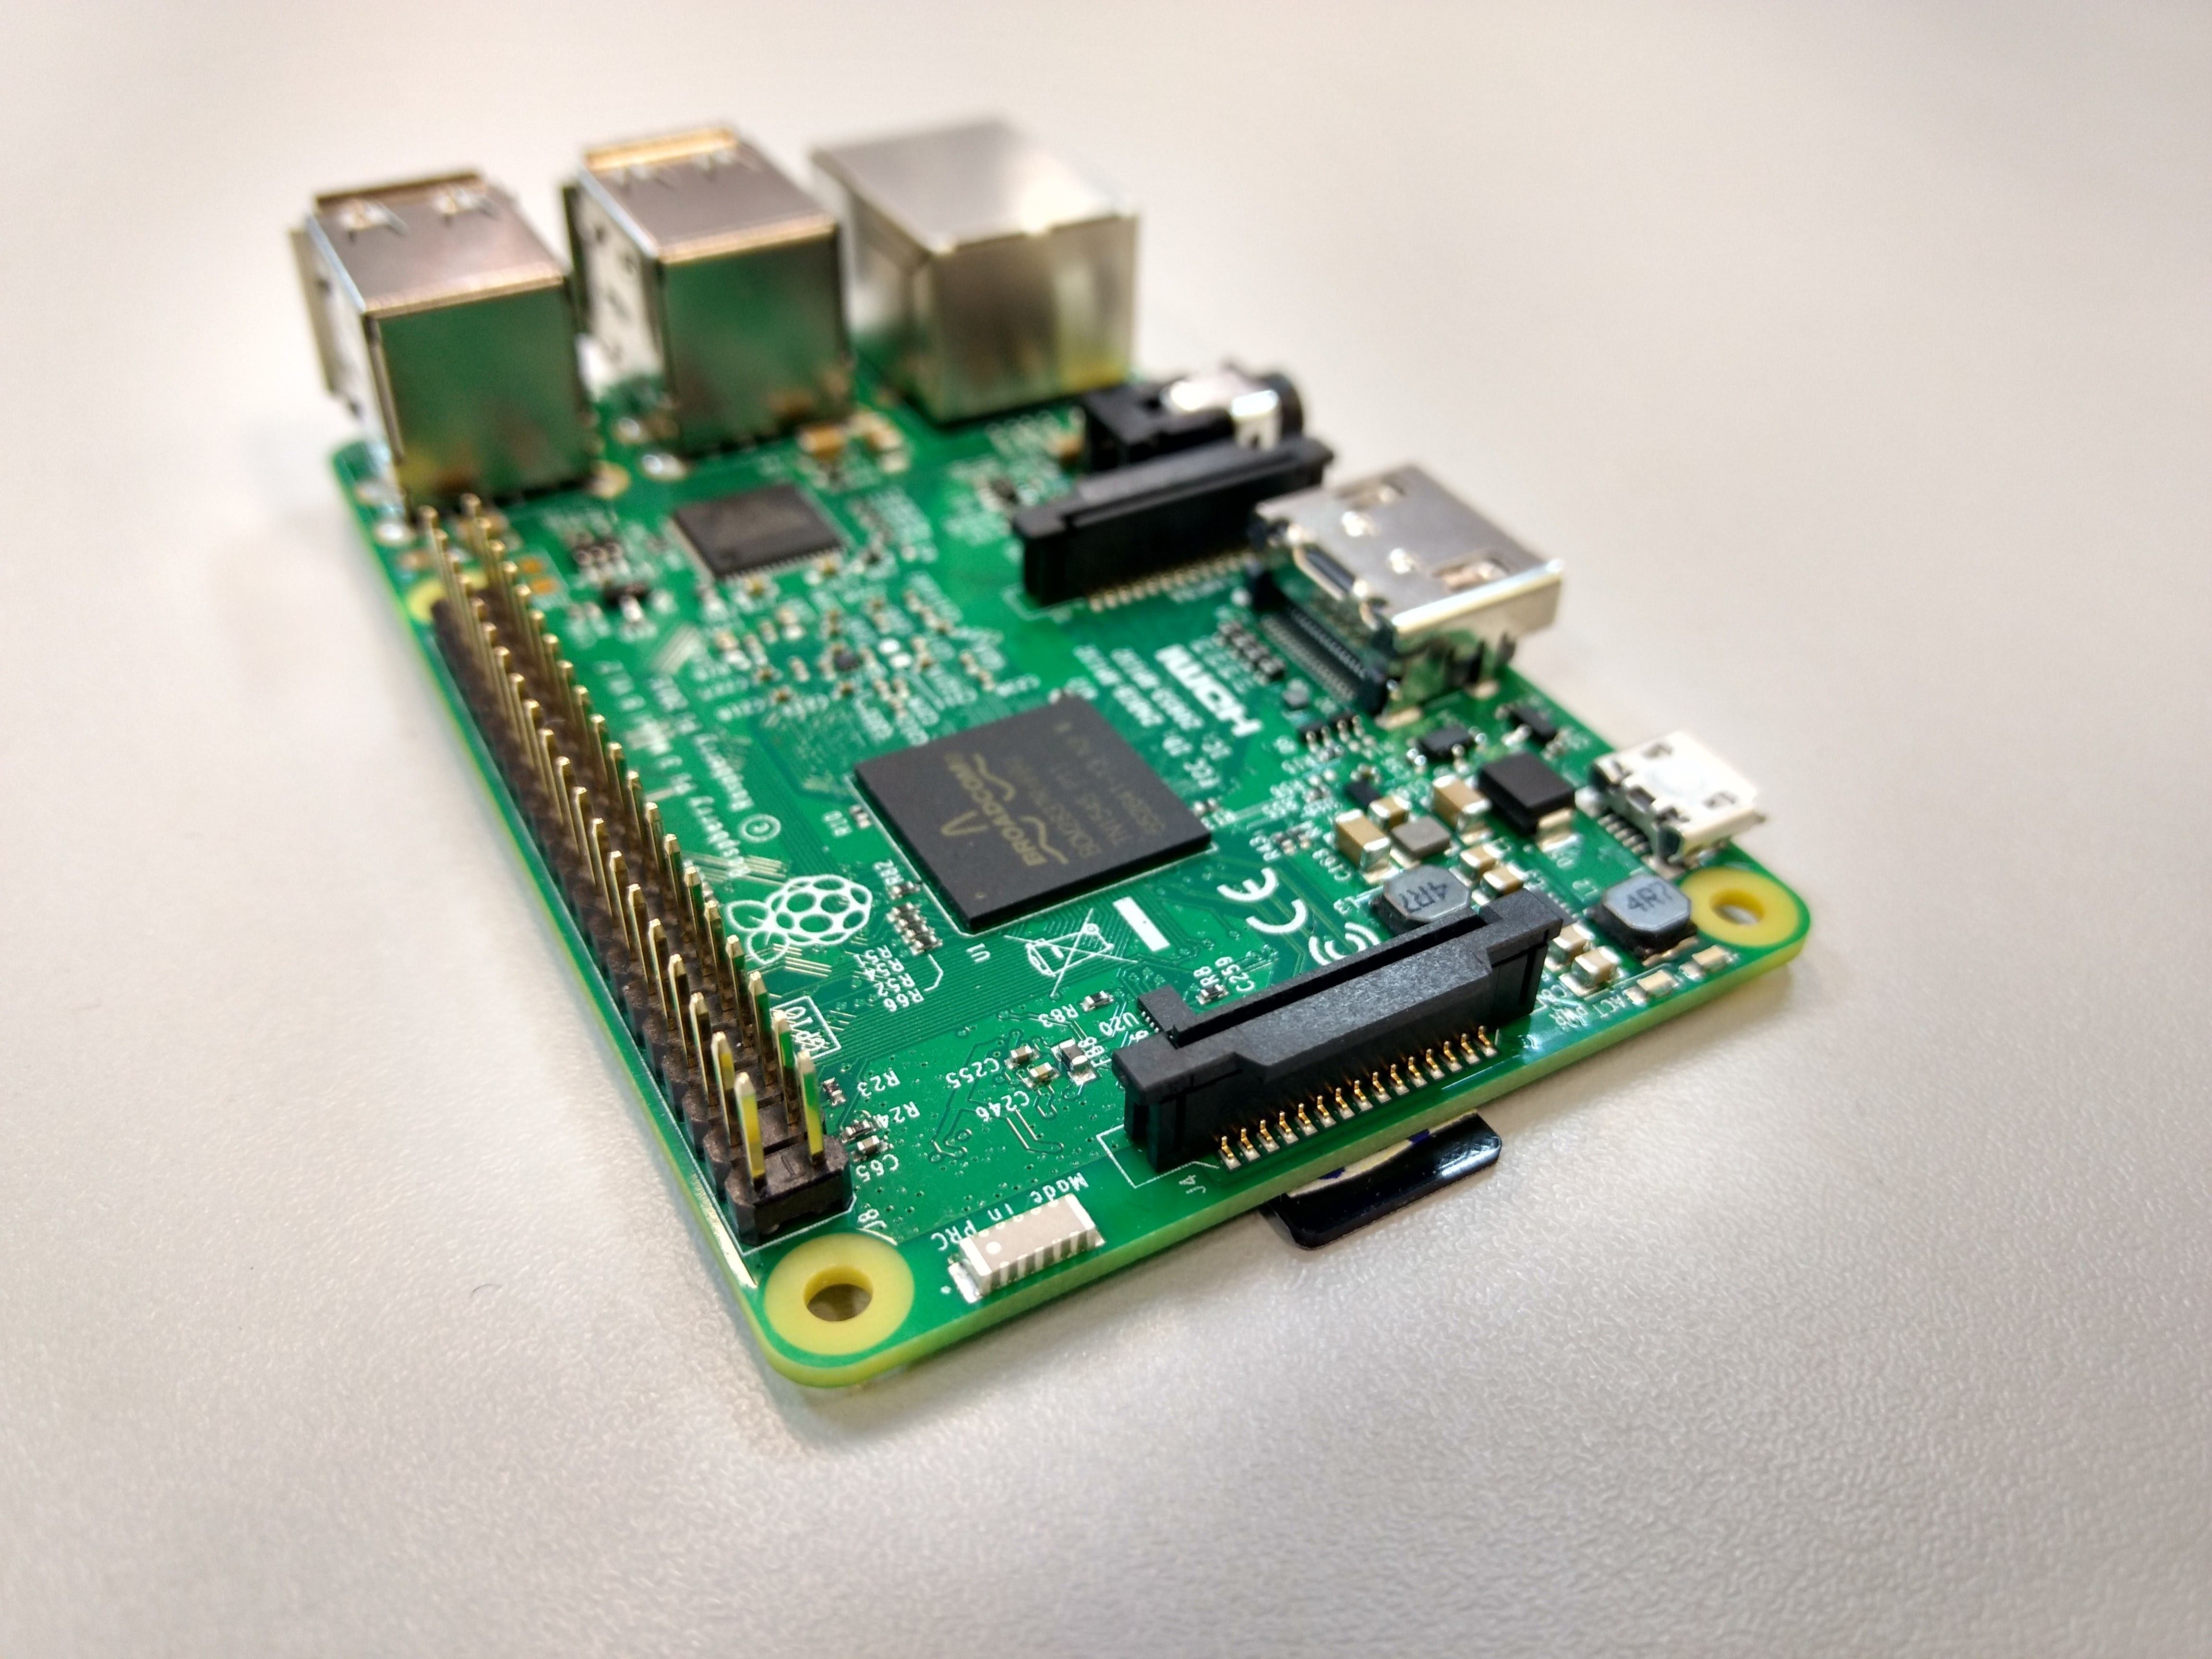
\includegraphics[width=1\textwidth]{040-plataformas/RPi-WiFi-dongles/rpi-onboard.jpg}
	\end{center}
	\legend{Fonte: Elaborada pelo autor}
\end{figure}



\subsection{Disponibilidade no mercado}
\label{subsec:mercado-rpi}

Para abordar a disponibilidade no mercado devemos também contar os periféricos
que são necessários para desenvolver na plataforma  RPi3 da mesma maneira que
foi feito com o ESP8266.

O RPI3 é ligado por uma fonte de 2A, 5V e 10W através de uma entrada micro
USB. Para ligá-lo, foi adquirido uma fonte USB tipo A para iPad, pois além de
poder desconectar o cabo da fonte, facilitando a manutenção, fornece a
quantidade exata de amperagem que o computador precisa. A primeira aquisição foi
de um carregador de \emph{smartphone} que não forneceu os amperes necessários.

Em comparação com a anterior, esta plataforma tem uma exigência energética maior,
muito disto é devido a \emph{Wi-Fi} integrado que é um destaque.
A antena de cerâmica do adaptador integrado pode ser vista no primeiro plano da
\autoref{fig-rpi-3}. Contudo, o adaptador não possui modo promíscuo e fez-se
necessário o uso de adaptadores \emph{Wi-Fi} USB. As recomendações da comunidade
quanto a escolha do adaptador USB (também conhecido como \emph{dongle Wi-Fi})
são o \emph{Edimax EW-7811Un} que não é tão comum no Brasil e o
\emph{EDUP EP-N85xx} que tem muitos genéricos no mercado nacional.

Como camada de \emph{software}, o RPi3 comporta diversos sistemas operacionais que são carregados de seu
cartão \emph{microSD}. Alguns exemplos de sistemas compatíveis são
\emph{Archlinux}, \emph{OpenELECE}, \emph{Raspbian}, \emph{Risc OS},
\emph{Pidora}, \emph{Kali Linux}, \emph{Windows 10 IoT}, entre outros. Para este
trabalho, foi utilizado o \emph{Raspbian}.

Portanto, para funcionamento e desenvolvimento de aplicações com RPI3 são
necessários componentes extra que são  demonstrados na
\autoref{table:custo-rpi}.

\begin{table}[htb]
\IBGEtab{%
\ABNTEXchapterfont {
	\caption{\label{table:custo-rpi}Descrição e custos com Raspberry Pi 3}%
}
}{%
\begin{tabular}{ccc}
\toprule
Produto								&	Descrição e utilização					&	Custo		\\
\midrule \midrule
Novo Raspberry Pi 3 (pi3)			&											&			 	\\
Quadcore 1.2ghz (10x+rapido) 1gb	&	Computador hospedeiro do sensor			&	R\$ 269,99	\\
\midrule
Fonte Carregador Original Usb		&	Fonte com conector USB tipo A que		&				\\
Apple Iphone 3 4 4s Ipad 1 2		&	supriu o consumo elétrico do RPI3		&	R\$ 13,99	\\
\midrule
Cabo USB com conectores 			&											&				\\
\emph{A} e \emph{Micro-B} 			&	Para conectar a fonte ao RPI3			&	R\$ 2,00^{1}	\\
\midrule
Cartão Micro Sdhc 16gb Ultra Sd 	&	Armazena o SO e outros arquivos, a		&				\\
Sandisk Classe 10 30mb/s			&	classe indica a velocidade do cartão	&				\\
									&	que implica na velocidade do SO			&	R\$ 21,99	\\
\midrule
Mini Adaptador Wireless Wifi 		&	Adaptador externo Wi-Fi que  			&				\\
Edup Usb 150mbps Raspberry Pi		&	permite modo promíscuo					&	R\$ 16,88	\\
\midrule
\bottomrule
\end{tabular}%
}{%
	\fonte{Produzido pelo autor.}%
	\nota[Nota 1]{Os cabos USB foram reutilizados de outras aplicações.}%
}
\end{table}


\subsection{Desenvolvimento e Implantação}
\label{subsec:devel-rpi}

Para desenvolver com o RPI3 é necessário instalar um sistema operacional
em seu cartão SD,  esse processo é simplificado com o uso do \emph{bootloader noobs}
pode ser encontrado no site oficial do respirar Prime  para download.  após
feito download os arquivos são extraídos do arquivo comprimido e colocados  na
pasta raiz do cartão SD.  o próximo passo é ligar a fonte ao responder,
colocar o cartão SD,  conectar monitor teclado e mouse ligar a fonte na tomada
para que imediatamente o computador ligue  e a tela escolha do sistema
operacional seja apresentada.    Nela deve escolher uma rede com ou sem fio para
conectar-se à internet e,  após conectado E é possível escolher o sistema
operacional que será baixado é instalado no próprio cartão SD.

O sistema operacional escolhido para a construção da plataforma de sensor É o
raspbian que é a distribuição Linux recomendada para o RPI. Nela já estão
instaladas e configuradas muitas ferramentas utilizadas para desenvolvimento e
implementação de projetos como git, ssh e nodejs que foram utilizados para a
construção da aplicação como discutido no próximo capítulo.

Para tornar o sistema completamente funcional para o desenvolvimento é
necessário somente executar os passos de segurança  e dar acessibilidade remota
ao sistema. Na interface gráfica de configuração do raspbian  deve ser alterado
a senha do usuário ‘pi’  e ativado serviço SSH que permite acesso remoto através
de um terminal.  os últimos três passos  são a atualização da lista de pacotes,
a atualização dos pacotes instalados e uma reinicialização do sistema  para
garantir o bom funcionamento e segurança do mesmo.

Feito isto qualquer desenvolvimento e implantação pode ser realizado com riscos
e falhas minimizados. Este processo é fundamental para a segurança da aplicação,
usuários e construtores pois, como foi revelado após os ataques de 21 de Outubro
de 2016, dispositivos IoT atualmente não oferecem estes níveis mínimos de
segurança (\emph{software} atualizado e senhas seguras) tornando-se um terreno
fértil para a construção de \emph{botnets} como foi o caso do \emph{malware
Mirai} utilizado para infectar milhares de dispositivos e causar o maior ataque
\emph{DDoS} até o momento com 1,2 terabits por segundo
\cite{guardianMirai} \cite{nytimesMirai}.


\subsection{Testes e resultados}
\label{subsec:testes-rpi}

De maneira análoga à feita com o ESP8266 analisamos a capacidade do Raspberry Pi
de operar com sua Wi-Fi em modo promíscuo porém,  devido  a diferença de camada
de software envolvida diferentes ferramentas foram utilizadas.

Neste caso utilizamos as ferramentas airodump e tshark além das ferramentas de
Wi-Fi padrões do sistema operacional \emph{raspbian}. Para verificar o modo
promíscuo no ambiente raspbian utiliza-se os comandos \emph{ifconfig},
\emph{iwconfig} e \emph{iw}, que são padrão do sistema operacional Debian, como
demonstrado a seguir.

\begin{verbatim}
pi@sensor-01:~ $ sudo ifconfig wlan0 down
pi@sensor-01:~ $ sudo iwconfig wlan0 mode monitor
pi@sensor-01:~ $ sudo ifconfig wlan0 up
\end{verbatim}

Este processo é
O resultado pode ser observado com o comando

\begin{verbatim}
pi@sensor-01:~ $ sudo iwconfig wlan0
wlan0   IEEE 802.11bgn  Mode:Monitor  Frequency:2.412 GHz  Tx-Power=20 dBm
        Retry short limit:7   RTS thr:off   Fragment thr:off
        Power Management:off
\end{verbatim}

Quando este processo foi realizado utilizando somente o adaptador de Wi-Fi
integrado no RPI3, cuja antena de cerâmica pode está em destaque na
\autoref{fig-rpi-onboard} o resultado foi negativo portanto outros adaptadores
foram necessários.

No ambiente do laboratório encontramos adaptadores \emph{Wi-Fi USB D-link}
(\autoref{fig-dlink}), porém executando o mesmo teste neles não foi possível
Ativar o modo promíscuo. Com um colega de laboratorio, pudemos emprestar um
terceiro adaptador, este do modelo \emph{Edup} (\autoref{fig-ralink-epub}) com
fabricanteidentificado por software de nome \emph{Ralink}, que teve resultado
positivo. Para a construção dos dois sensores foi necessária a aquisição, e
subsequente teste, de mais um modelo de adaptador que está listado na
\autoref{table:custo-rpi} que também tem fabricante \emph{Ralink} porém a sua
aparência externa difere do anterior e pode ser visualizada na
\autoref{fig-ralink}, mesmo que a aquisição foi do mesmo anúncio.

\begin{figure}[htb]
 \label{adaptadores-usb}
 \centering
  \begin{minipage}{0.49\textwidth}
    \centering
    \caption{Antena cerâmica de Wi-Fi e Bluetooth do Raspberry Pi 3 \label{fig-rpi-onboard}}
    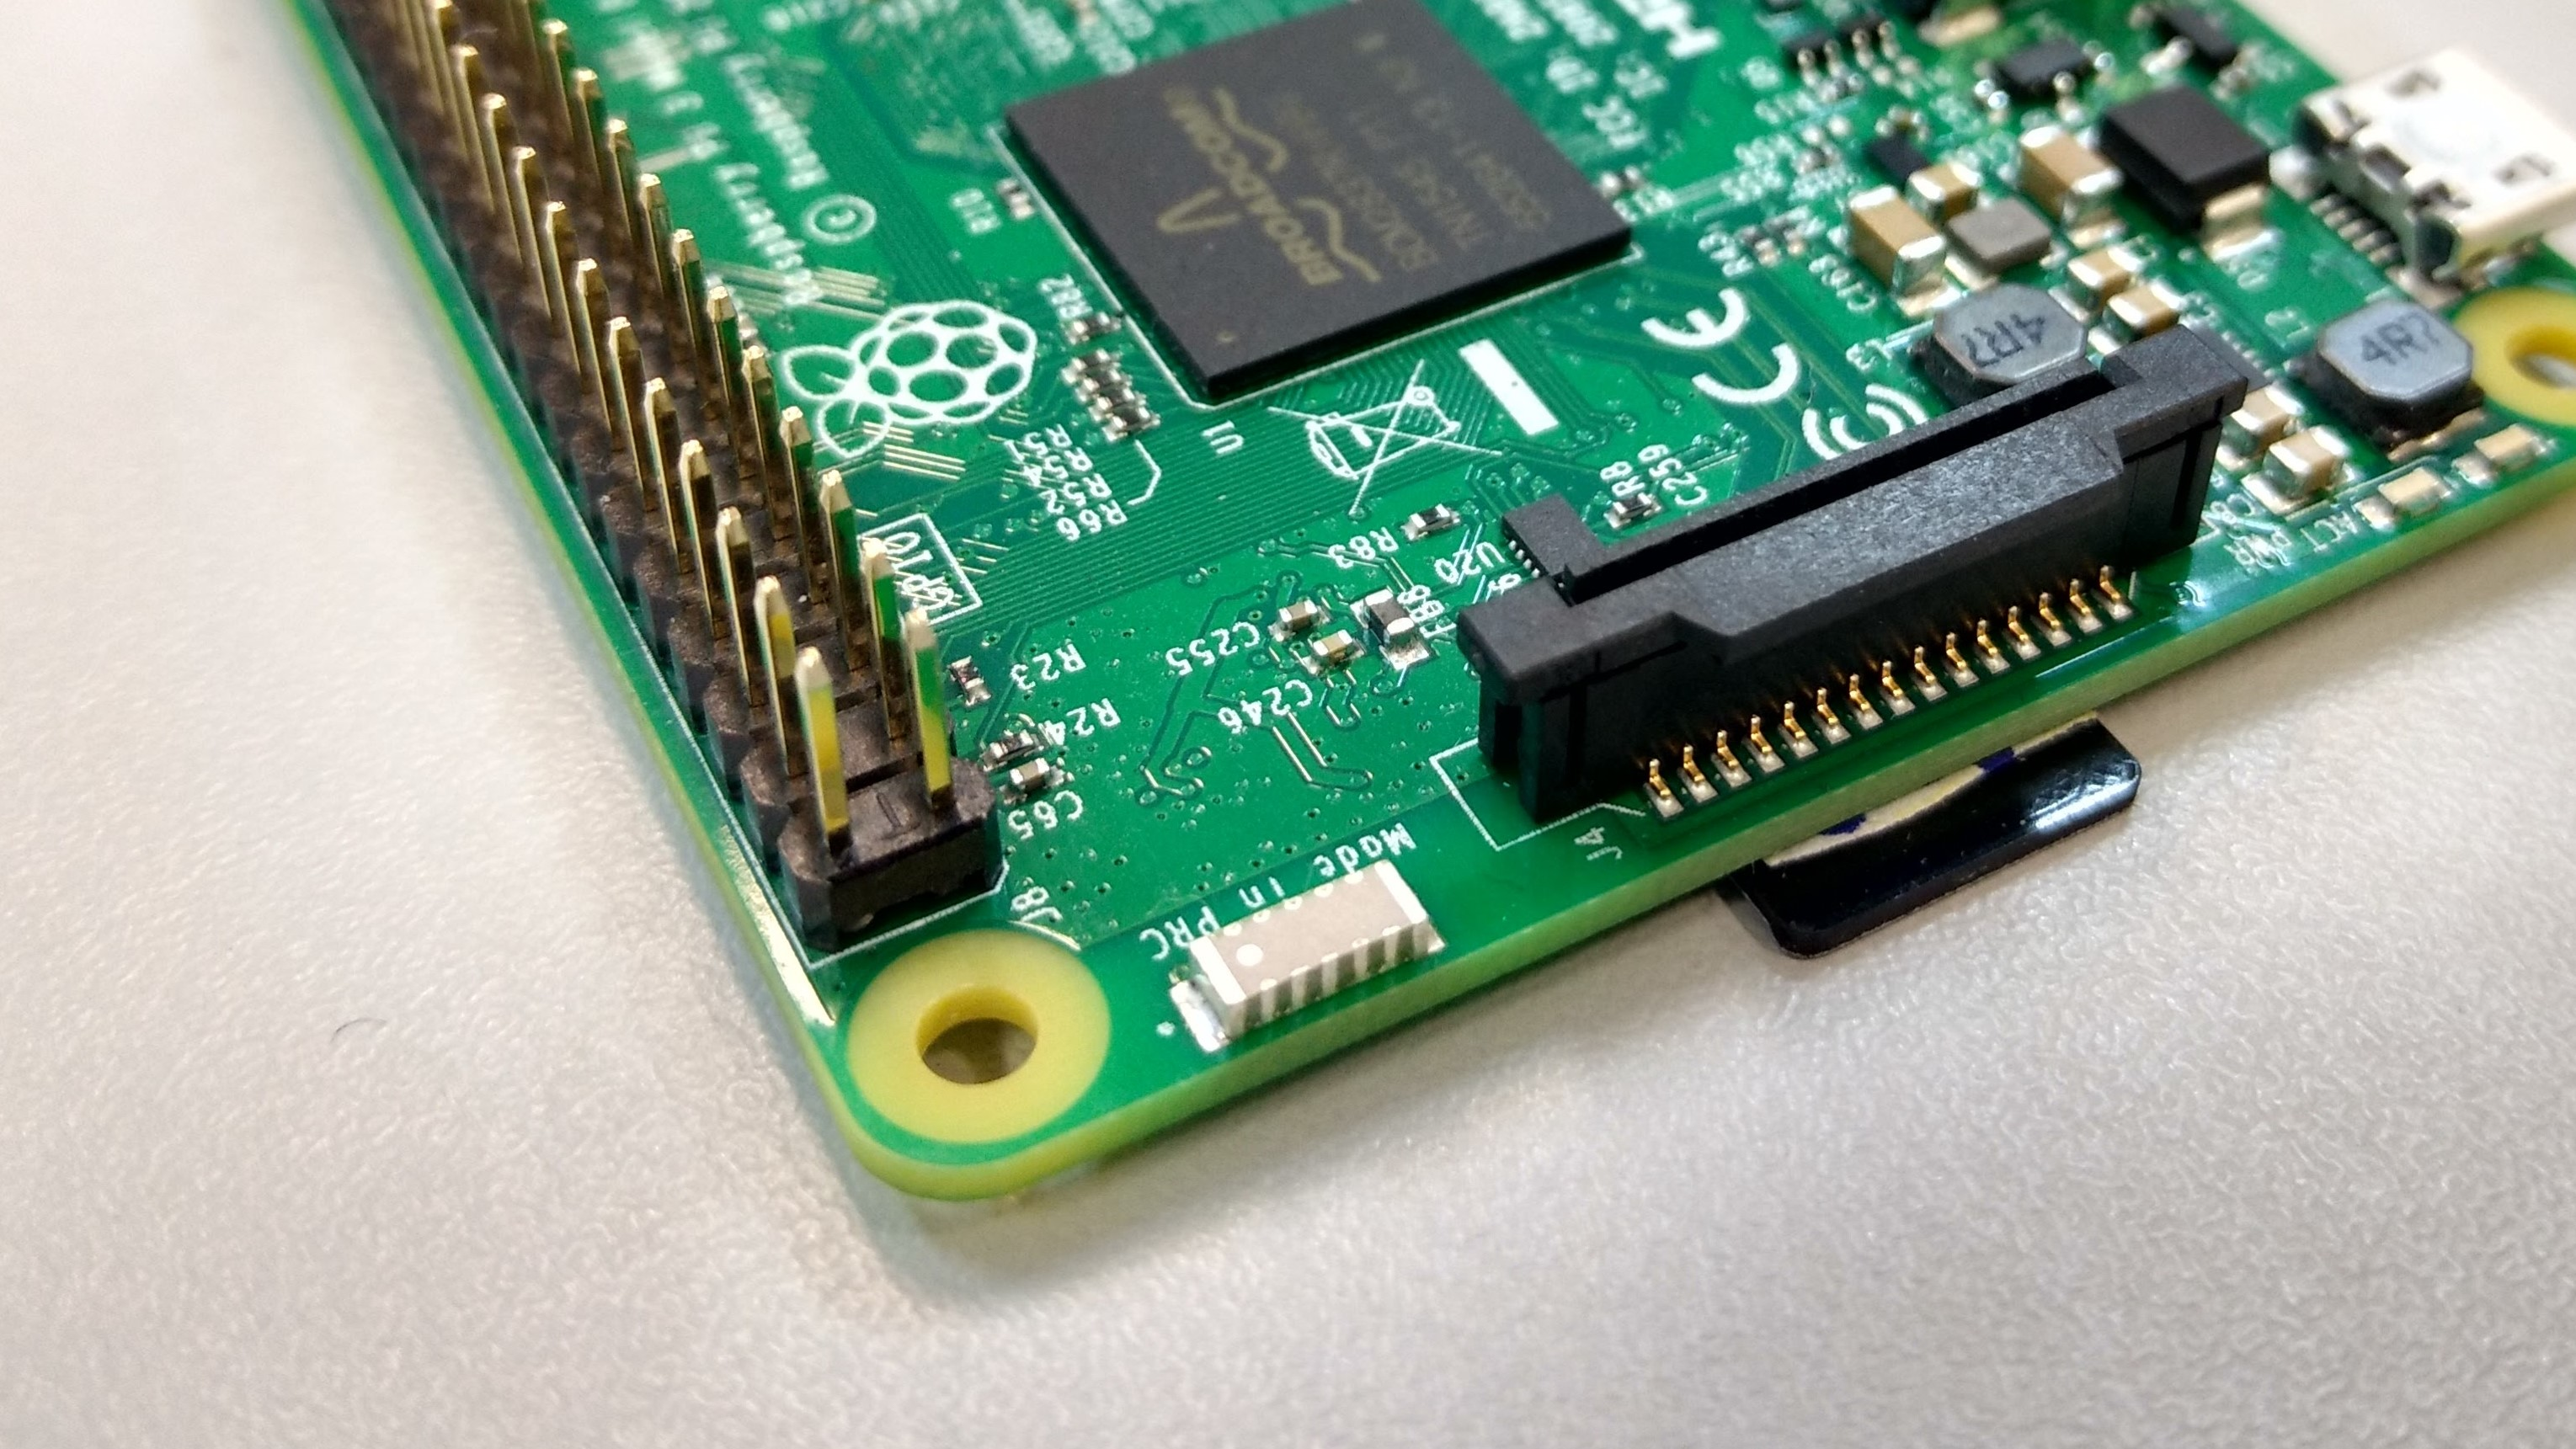
\includegraphics[width=1\textwidth]{040-plataformas/RPi-WiFi-dongles/cut_rpi-onboard.jpg}
    \legend{Fonte: Produzido pelos autores}
  \end{minipage}
  \hfill
  \begin{minipage}{0.49\textwidth}
	\centering
  	\caption{Adaptador Wi-Fi USB D-Link do laboratório \label{fig-dlink}}
  	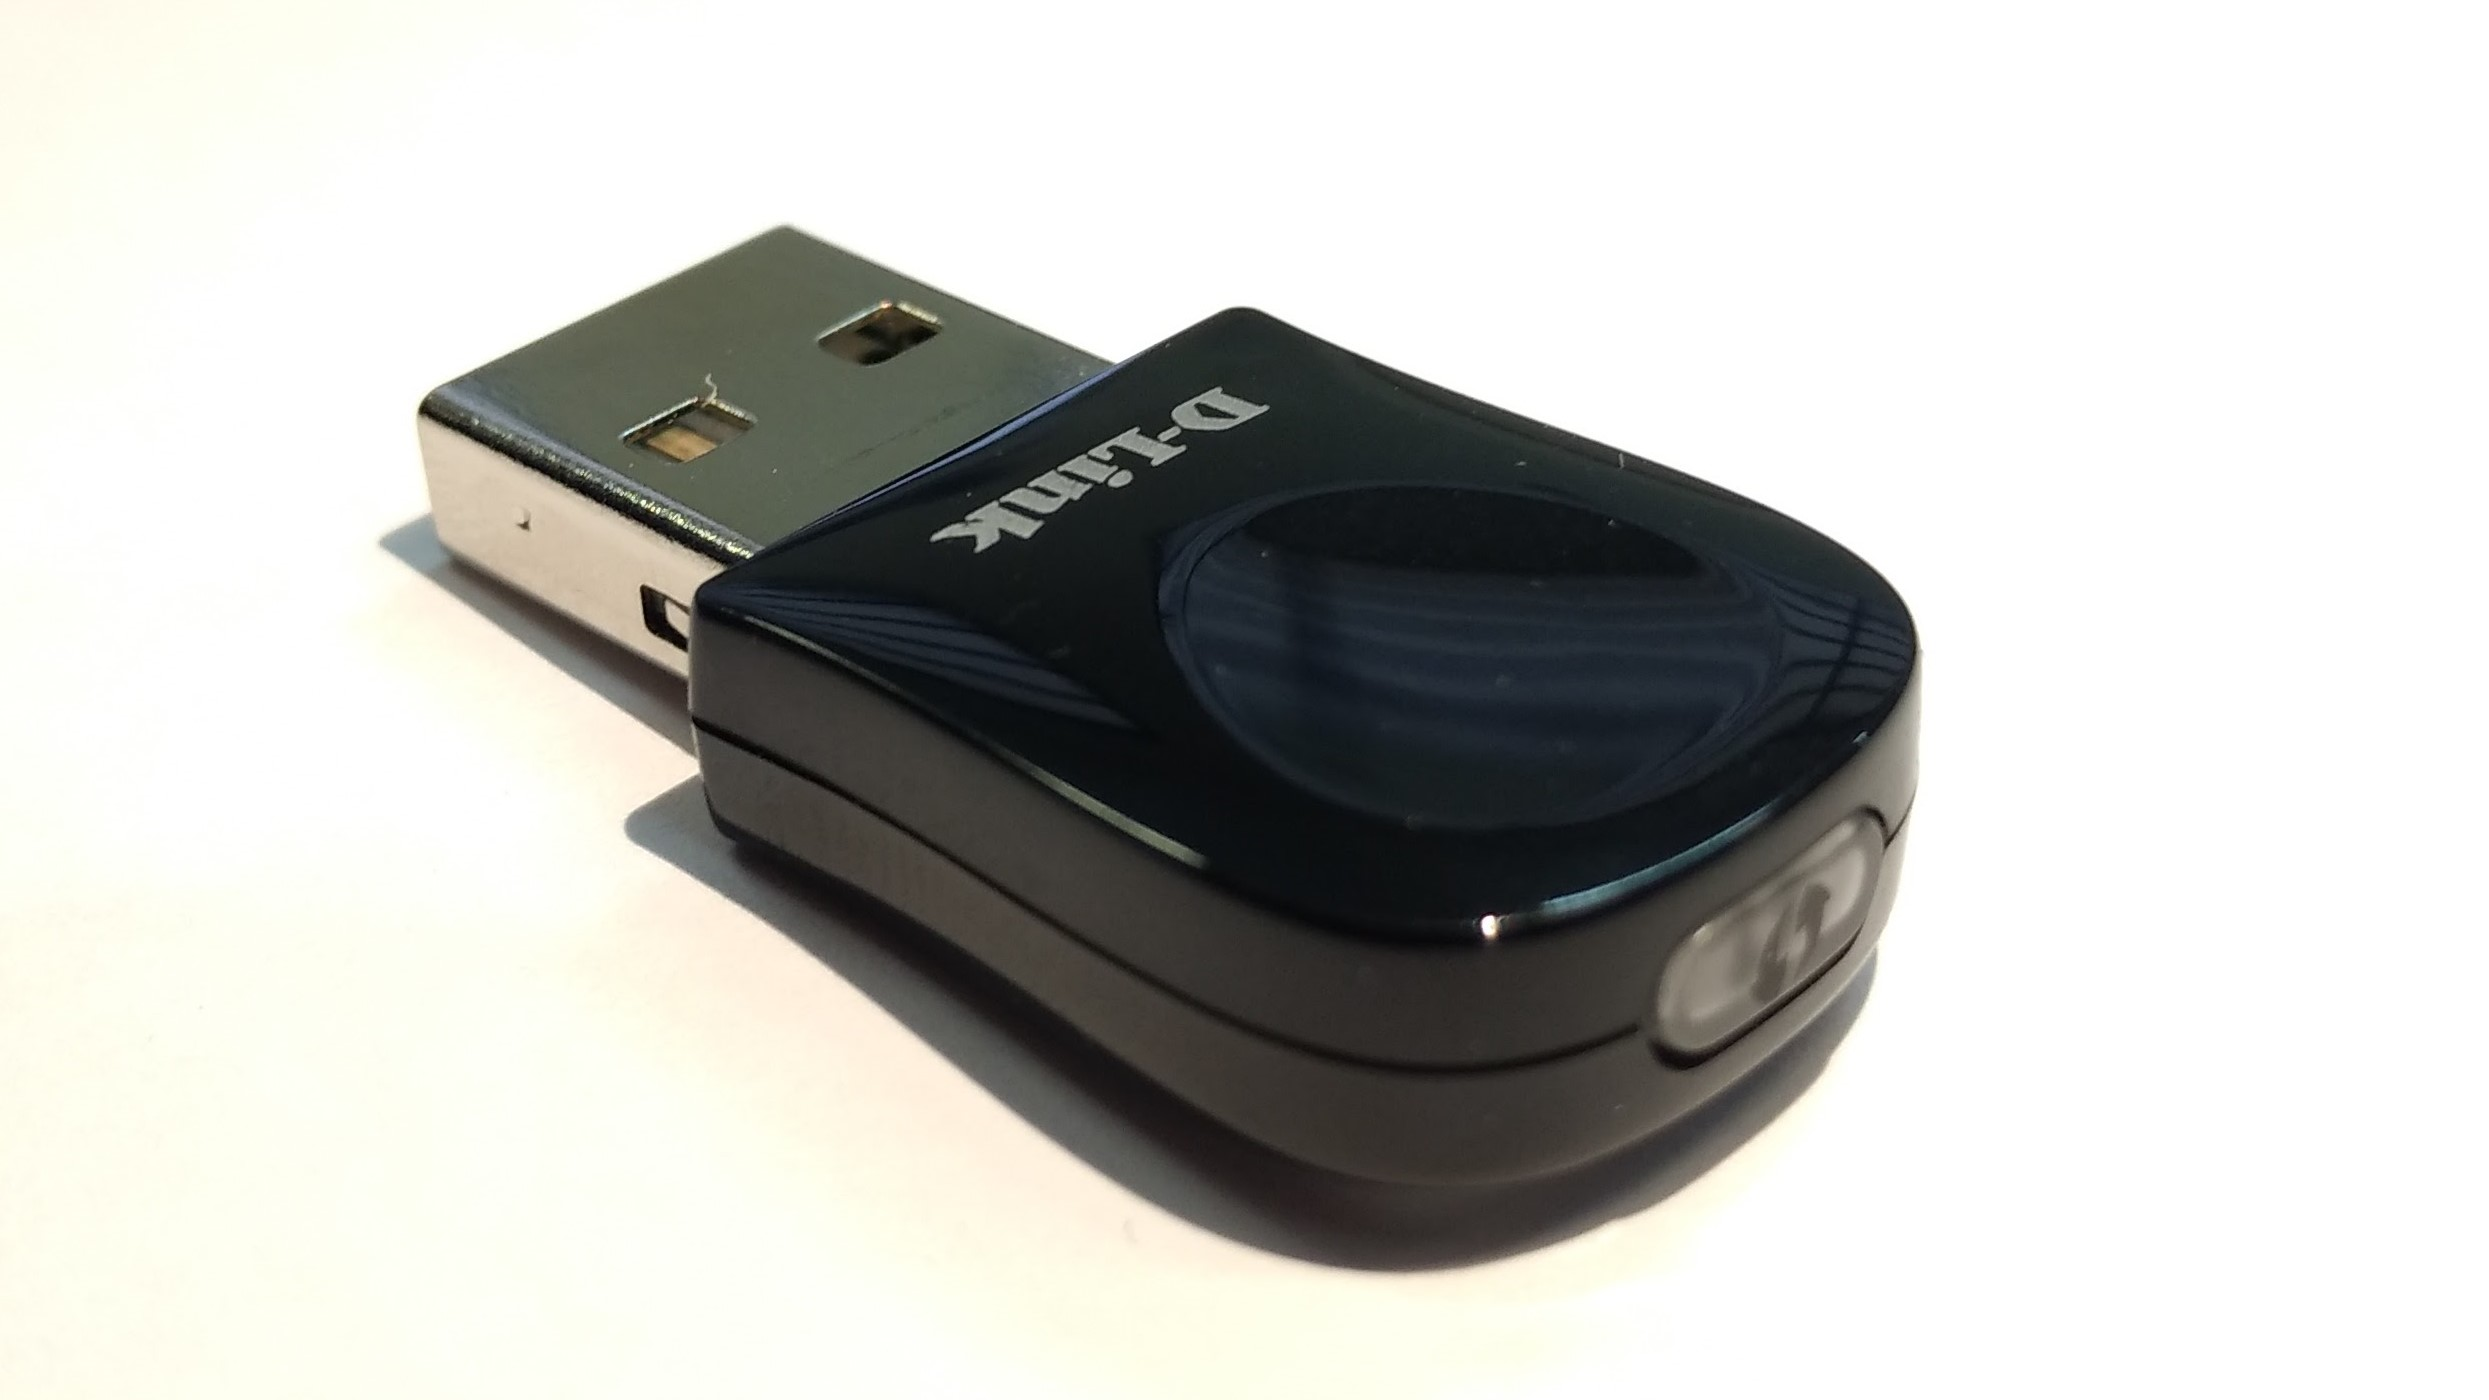
\includegraphics[width=1\textwidth]{040-plataformas/RPi-WiFi-dongles/cut_dlink.jpg}
  	\legend{Fonte: Produzido pelos autores}
  \end{minipage}
\end{figure}

\begin{figure}[htb]
 \label{adaptadores-usb-2}
  \begin{minipage}{0.45\textwidth}
	  \centering
	  \caption{Adaptador Wi-Fi USB Ralink Epub emprestado \label{fig-ralink-epub}}
	  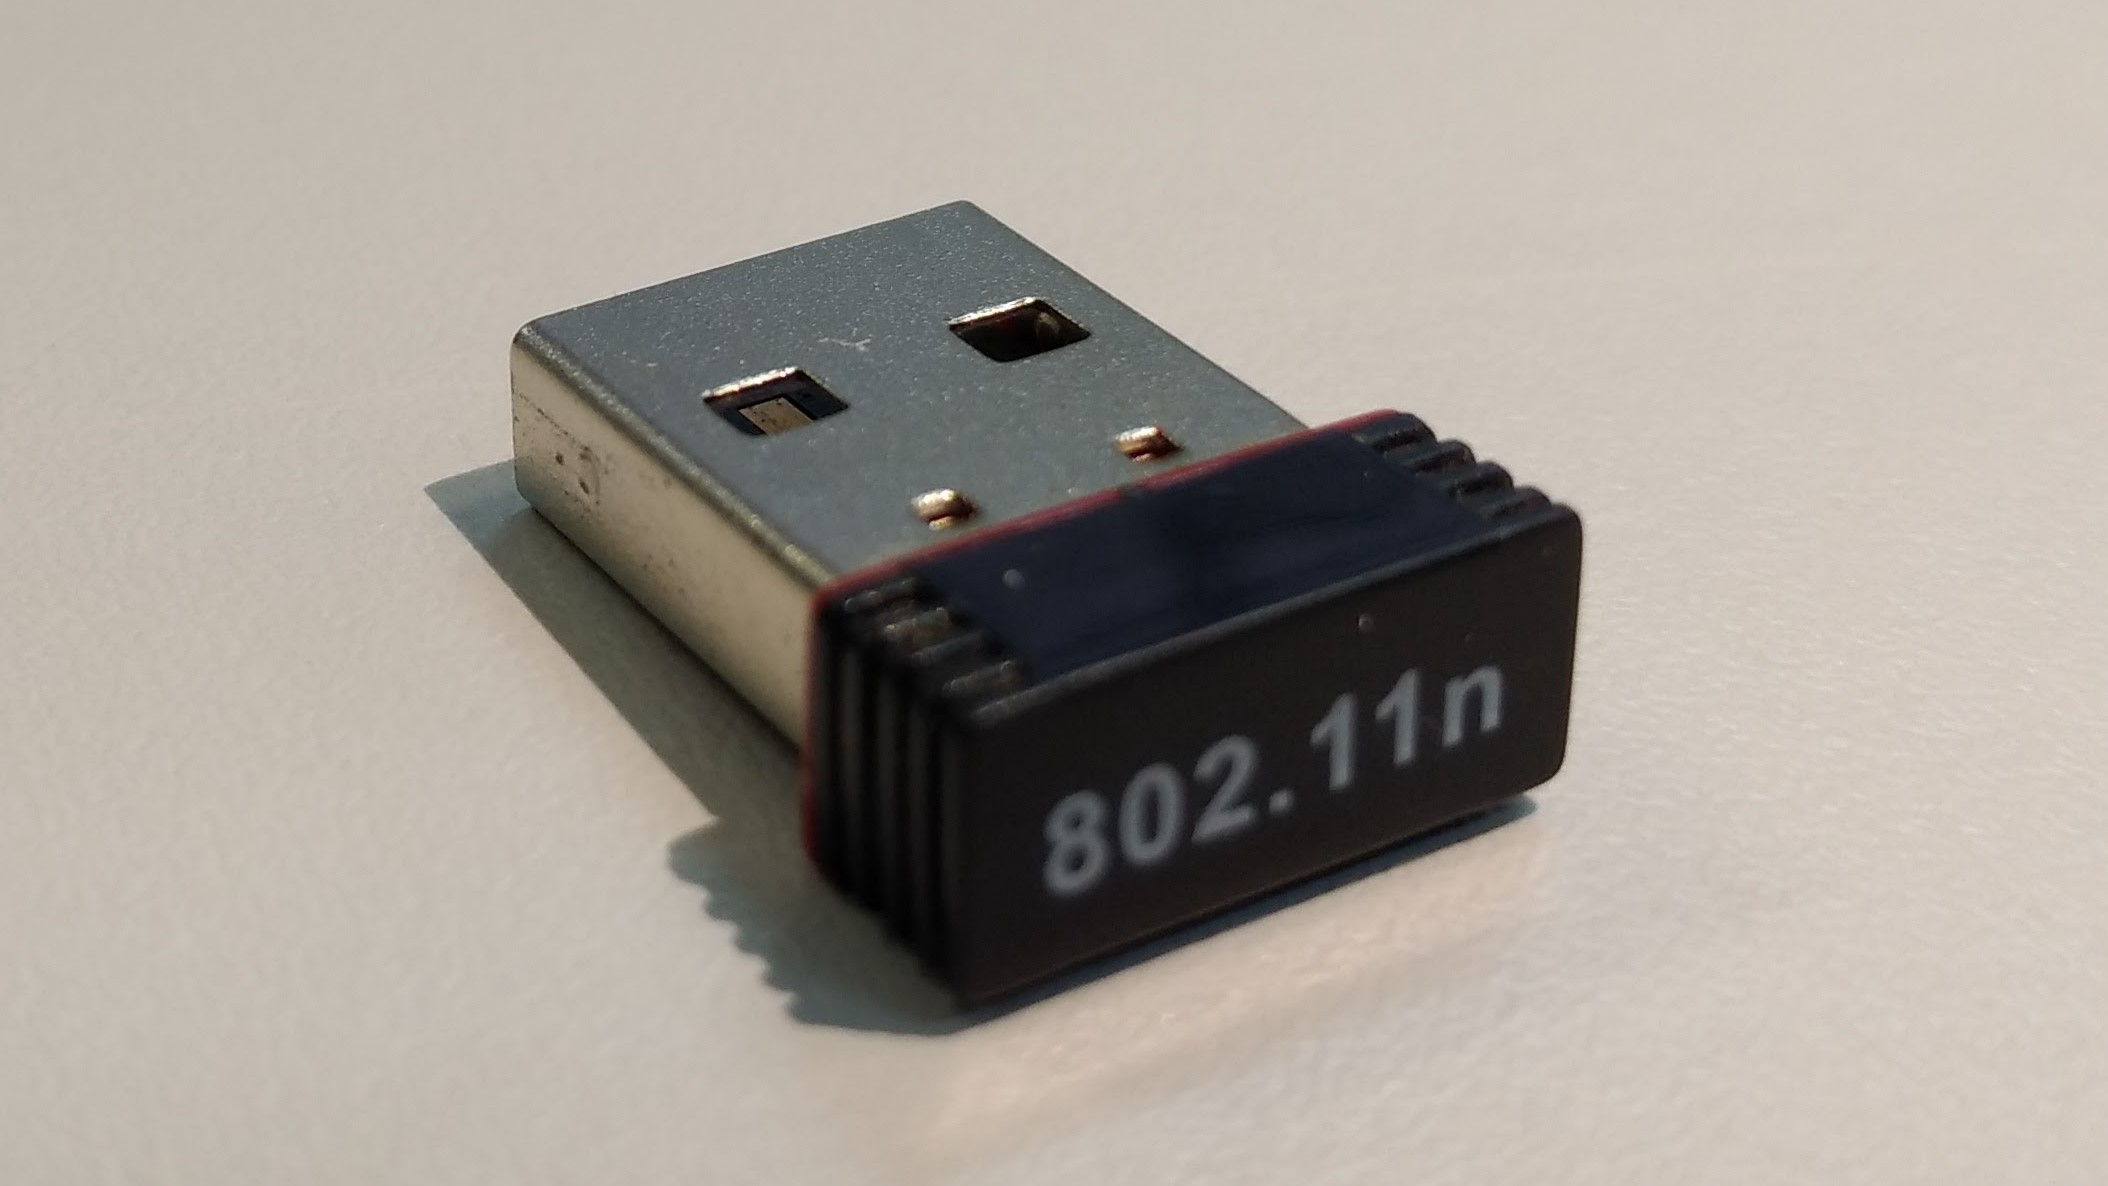
\includegraphics[width=1\textwidth]{040-plataformas/RPi-WiFi-dongles/cut_ralink-epub.jpg}
	  \legend{Fonte: Produzido pelos autores}
  \end{minipage}
  \hfill
  \begin{minipage}{0.45\textwidth}
	  \centering
	  \caption{Adaptador Wi-Fi USB Ralink Epub comprado \label{fig-ralink}}
	  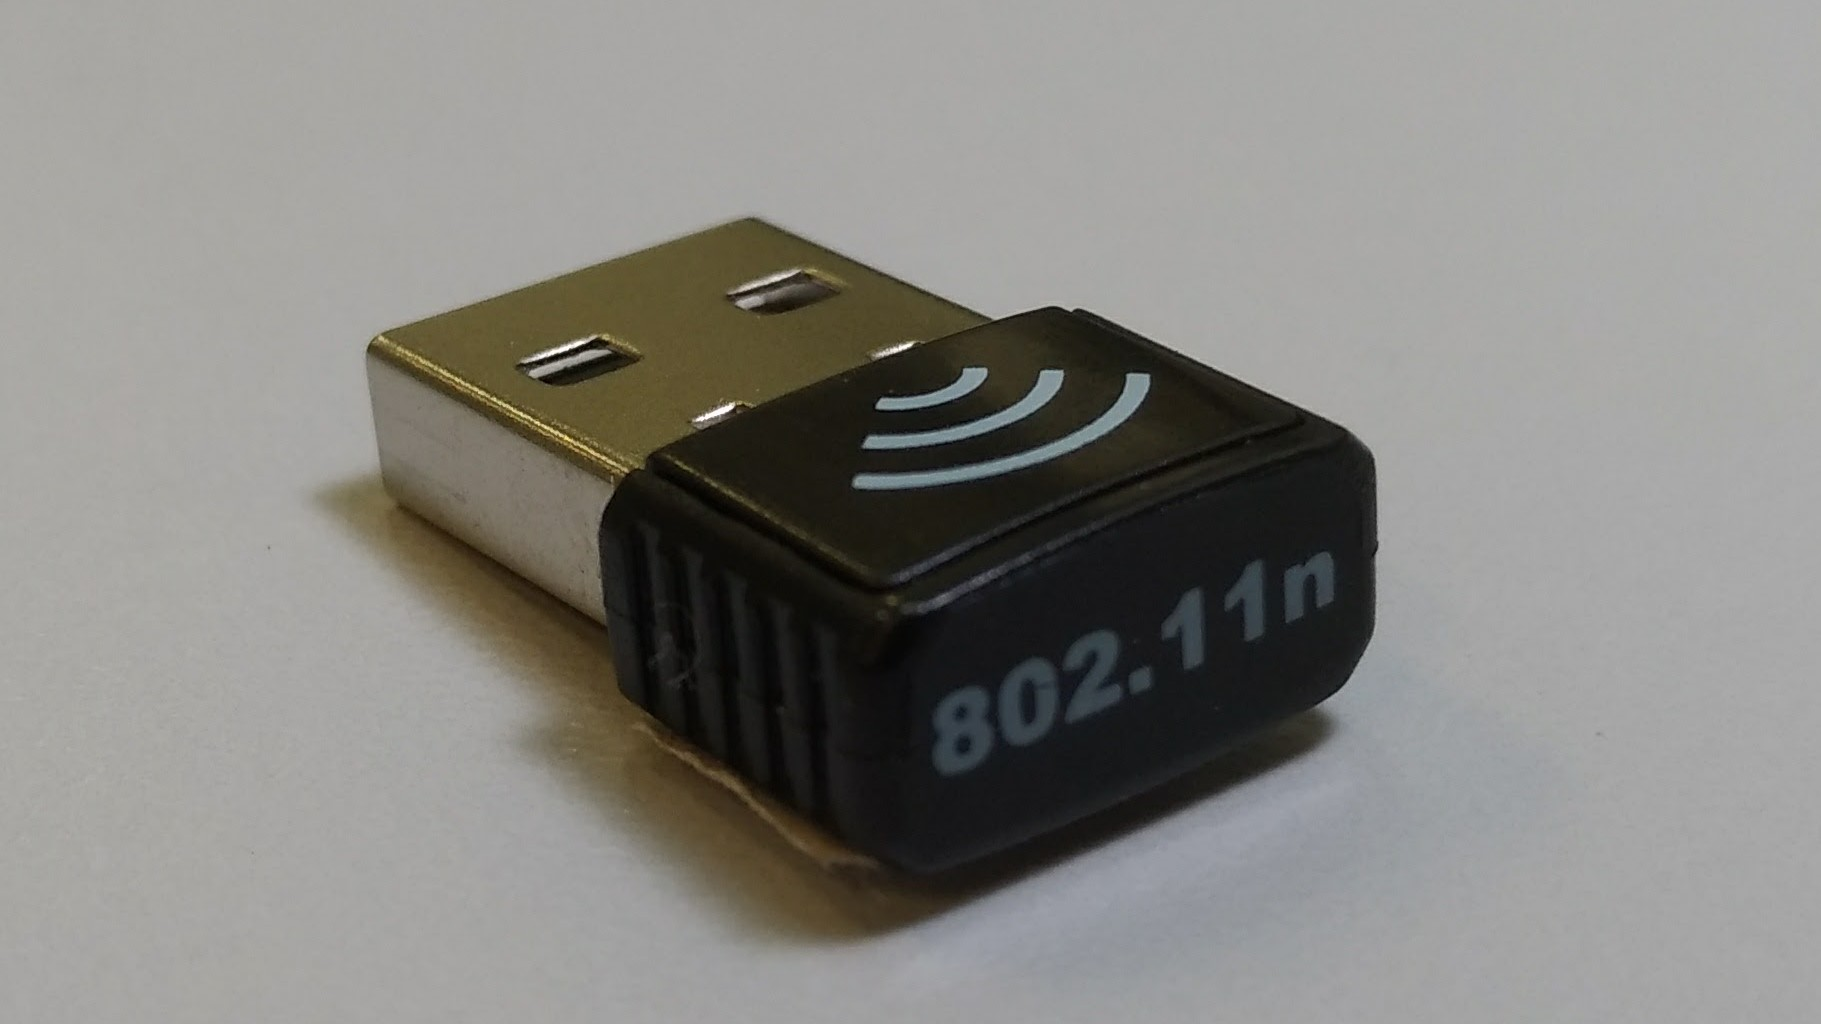
\includegraphics[width=1\textwidth]{040-plataformas/RPi-WiFi-dongles/cut_ralink.jpg}
	  \legend{Fonte: Produzido pelos autores}
  \end{minipage}
\end{figure}


Para capturar e avaliar pacotes É necessário uma ferramenta  para tal. Na área
de segurança da informação podemos encontrar \emph{airodump} que é utilizado para
avaliar e explorar vulnerabilidades de segurança em redes Wi-Fi. Outra área que
forneceu uma ferramenta adequada é a área de qualidade de serviço em redes de
computadores onde o \emph{software Wireshark} é bem popular, uma interface alternativa
do mesmo feita para uso em terminal é chamada \emph{tshark}.

Para testar a viabilidade do sensor utilizou-se \emph{airodump} que é uma
ferramenta de terminal interativa como vista na \autoref{fig-airodump} onde é
demonstrado a capacidade de capturar pacotes do tipo \emph{Beacon} (tabela com
BSSID, PWR e Beacons na parte superior da \autoref{fig-airodump}) que anunciam
a presença de AP (\emph{Access Point} - ponto de acesso) e o nome da rede que
ele está servindo e, também os pacotes entre os dispositivos (\emph{Stations})
associados a um AP (tabela com BSSID, STATION e PWR na parte inferior da
\autoref{fig-airodump}). Em ambos os casos é mostrado um valor de potência de
sinal (PWR) associado a cada transmissor portanto, demostrando a viabilidade
do sensor com a informação de potência de sinal.

\begin{figure}[htb]
	\caption{\label{fig-airodump}Interface do airodump-ng}
	\begin{center}
	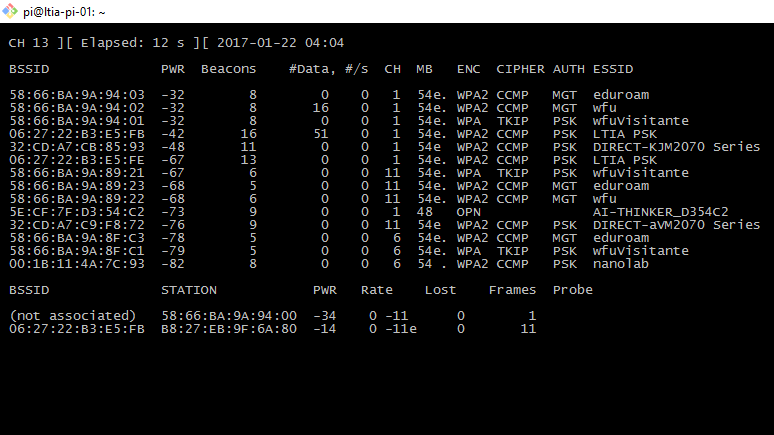
\includegraphics[width=1\textwidth]{040-plataformas/RPi-WiFi-dongles/wifi-sniff-rpi/4-rpi-airodump.png}
	\end{center}
	\legend{Fonte: Elaborada pelo autor}
\end{figure}


**Conclusão sobre Raspberry Pi**

O Raspberry foi adotado como o sensor para detectar os dispositivos. O modo
promíscuo conseguiu ser acessado através de adaptador/módulo USB Wi-Fi. Mais
detalhes sobre a construção e adoção deste computador serão apresentados no
capítulo "Construção".

**Comparativo RPi X ESP8266**

Em comparação com o ESP8266, o Raspberry Pi compensou seu custo mais caro devido
a facilidade de programação e acesso aos seus recursos e integração e acesso a
recursos externos. Além disso, foi possível chegar ao modo promíscuo facilmente
através do Bash e do sistema operacional. A seguir, uma tabela comparando as
principais características do RPi e do módulo ESP12F.

\begin{figure}[htb]
	\caption{\label{fig-raspbian-jessie}Raspbian Jessie com Pixel}
	\begin{center}
		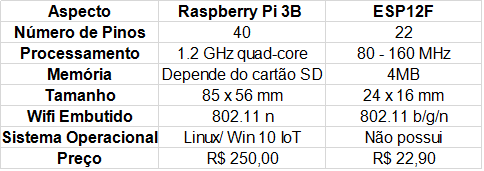
\includegraphics[width=1\textwidth]{040-plataformas/Plataformas DIY e comparacao/rpi-esp.png}
	\end{center}
	\legend{Fonte: Elaborada pelo autor}
\end{figure}
